% !TEX encoding = UTF-8 Unicode

\documentclass[a4paper]{article}

\usepackage{color}
\usepackage{amsmath}
\usepackage{url}
\usepackage[T2A]{fontenc} % enable Cyrillic fonts
\usepackage[utf8]{inputenc} % make weird characters work
\usepackage{graphicx}

\usepackage[english,serbian]{babel}
%\usepackage[english,serbianc]{babel} %ukljuciti babel sa ovim opcijama, umesto gornjim, ukoliko se koristi cirilica
\usepackage{listings}
\usepackage{minted}
\usepackage[unicode]{hyperref}
\hypersetup{colorlinks,citecolor=green,filecolor=green,linkcolor=blue,urlcolor=blue}

%\newtheorem{primer}{Пример}[section] %ćirilični primer
\newtheorem{primer}{Primer}[section]

\begin{document}

\title{Skripta za vežbe\\ \small{Skripta u okviru kursa\\Istraživanje podataka 2\\ Matematički fakultet}}

\date{24.~sept 2018.}
\maketitle


\tableofcontents

\newpage

\section{Uvod}
\label{sec:uvod}



\begin{primer}
Prvi primer služi kao podsetnik na određene mogućnosti koje nam pruža $pandas$ biblioteka.  
Najpre, importujemo biblioteku, potom uz pomoć $read\_csv$ vršimo učitavanje $.csv$ fajla koji sadrži podatke koje želimo da analiziramo i na kraju vršimo ispise različitih vrednosti.
\end{primer}
\inputminted{python}{Codes/1/pandas-example.py}
\begin{lstlisting}
  sepal_length  sepal_width  petal_length  petal_width    species
0        	  5.1          3.5           1.4          0.2     setosa
1             4.9          3.0           1.4          0.2     setosa
2             4.7          3.2           1.3          0.2     setosa
3             4.6          3.1           1.5          0.2     setosa
4             5.0          3.6           1.4          0.2     setosa
5             5.4          3.9           1.7          0.4     setosa
...
[150 rows x 5 columns]
______________________________________________________________________
sepal_length    float64
sepal_width     float64
petal_length    float64
petal_width     float64
species          object
dtype: object
Index(['sepal_length', 'sepal_width', 'petal_length', 'petal_width',
       'species'],
      dtype='object')
RangeIndex(start=0, stop=150, step=1)
[[5.1 3.5 1.4 0.2 'setosa']
 [4.9 3.0 1.4 0.2 'setosa']
 [4.7 3.2 1.3 0.2 'setosa']
________________________________________________________________________
     sepal_width  petal_length
0            3.5           1.4
1            3.0           1.4
2            3.2           1.3
3            3.1           1.5
4            3.6           1.4
...
[150 rows x 2 columns]
\end{lstlisting}


\subsection{Istraživanje Veba - Web Mining}
\label{sec:veb}
Kada posmatramo distribuirani sistem informacija, vidimo da su dokumenti i objekti najčešće povezani kako bi se omogućio interaktivni pristup. Glavni primer distribuiranog sistema je Veb, gde korisnici, u potrazi za informacijama, $"$putuju$"$ od objekta do objekta uz pomoć hiperlinkova i $URL$ adresa. Veb konstantno raste i svaki dan se dodaje po nekoliko miliona stranica. Sa ovakvim, neprekidnim, rastom dostupnih stranica i podataka uviđa se da dobijanje informacija iz takvih izvora postaje sve teže i teže. Kao jedan od glavnih problema pri analizi Veb stranica javlja se nedostatak strukture. Pod $"$rudarenjem  (istraživanje) Veba$"$ (engl. \em{web mining}) podrazumevamo korišćenje tehnika za $"$rudarenje (istraživanje) podataka$"$ (engl. \em{data mining}) kako bi se automatski otkrile i izvlačile informacije sa Veb dokumenata i servisa. Web mining možemo podeliti na četiri glavne celine:
\begin{enumerate}
\item pronalaženje resursa - prikupljanje informacija preko na primer Web stranica kao što su stranice sa vestima i slično,
\item odabir informacija i pretprocesiranje - različite vrste transformacija nad podacima: uklanjanje stop reči, dobijanje željene reprezentacije i drugo,
\item generalizacija - proces automatskog otkrivanja uobičajenih uzoraka (engl. \em{pattern}) korišćenjem različitih opštih tehnika mašinskog učenja, istraživanja podataka i raznih veb-orijentisanih metoda i  
\item analiza - vrši se validacija i/ili interpretacija istraženih uzoraka(engl. \em{mined patterns}) . 
\end{enumerate}
Jedna od mogućih podela istraživanja Veba odnosi se na to koji deo Veba neko želi da analizira. Postoje tri vida istraživanja Veba:
\begin{enumerate}
\item Istraživanje sadržaja Veba (engl. \em{Web content mining}) - koristi sadržaj Veb stranice kako bi prikupio podatke: tekst, slike, video ili bilo koji drugi sadržaj,
\item Istraživanje strukture Veba (engl. \em{Web structure mining}) - fokusira se na strukturu veza veb stranice,
\item Istraživanje upotrebe Weba (engl. \em{Web usage mining}) - kao podatke koristi podatke prikupljene od interakcija korisnika pri korišćenju interneta.
\end{enumerate}

Najčešća upotreba istraživanja sadržaja Veba je u procesu pretrage. Na primer, crawler-i se koriste od strane pretraživača da izvuku sadržaj Veb strane kako bi se odmah dobili traženi rezultati. Isto tako, oni se mogu koristiti tako da im fokus bude na određenoj temi ili oblasti interesovanja, umesto da zahtevaju sve informacije koje se mogu dostići.

Kako bi se kreirao fokusirani crawler, klasifikator se obično trenira na skupu podataka odabranih od strane korisnika, kako bi crawler znao koji tip sadržaja traži. Potom on identifikuje stranice od interesa kako na njih nalazi i prati dalje sve linkove sa te stranice. Ako linkovi sa neke stranice od interesa vode ka nekim drugim stranicama koje su klasifikovane kao stranice koje nisu od interesa onda se linkovi na tim stranama dalje ne posmatraju. Istraživanje sadržaja se može najlakše direktno videti u procesu pretrage. Svi veći pretraživači danas koriste strukturu koja podseća na listu. Ta lista je uređena uz pomoć algoritma za rangiranje stranica.\\\\

U $Pythonu$ postoji modul $sklearn.feature_extraction$ koji služi za izvlačenje objekata (engl. features) iz skupova podataka koji sadrže tekst ili slike, u formatu koji je podržan od strane algoritama mašinskog učenja. 

\subsubsection{Izvlačenje teksta}

Analiza teksta je jedna od važnih primena algoritama mašinskog učenja. Međutim, sirovi podaci (engl. \em{raw data}) predstavljaju prepreku utoliko što ih algoritmima ne možemo dati direktno, već nam je potrebna neka njihova numerička reprezentacija uz pomoć vektora fiksirane dužine. Kako bi se ovaj problem rešio $scikit-learn$ nudi nekoliko načina da se iz tekstualnog sadržaja izvuku numerički podaci, princip koji se koristi je sledeći:
\begin{itemize}
\item dodeljivanje tokena stringova i davanje $id$-ja za svaki od tokena, npr. korišćenjem razmaka ili zareza kao odvajajućih elemenata između dva tokena,
\item brojanje pojavljivanja tokena u svakom od dokumenata,
\item normalizacija i dodeljivanje težina sa smanjenjem bitnosti onih tokena koji se često pojavljuju
\end{itemize}
Korpus dokumenata se, dakle, može predstaviti uz pomoć matrice koja ima jedan red po dokumentu i jednu kolonu po tokenu (reči) koje se javljaju u korpusu.
\textbf{Vektorizacijom} nazivamo proces pretvaranja kolekcije tekst dokumenata u numeričke vektore objekata (engl. \em{numerical feature vectors}). Konkretna strategija navedena gore (tokenizacija, brojanje i normalizacija) naziva se \textit{Bag of Words} reprezentacija. Dokumenti su opisani pojavljivanjima reči ignorišući informacije o poziciji reči u dokumentima.\\\\

$CountVectorizer$ iz $sklearn.feature_extraction.text$ implementira i tokenizaciju i brojanje pojavljivanja u istoj klasi. Korišćenje $"$stop$"$ reči, poput $"$and$"$, $"$the$"$, itd., za koje se pretpostavlja da ne nose nikakve informacije u kontekstu teksta, mogu biti uklonjene. Nekada, međutim, može se desiti da su slične reči korisne za predikciju, tako da sa korišćenjem $"$stop$"$ reči treba biti oprezan. Jedna od najpoznatijih $"$stop$"$ lista reči je $"$english$"$.
U velikim korpusima teksta, neke reči će se ponavljati veoma često, samim tim takve reči ni ne nose puno značajnih informacija o stvarnom sadržaju dokumenta. Ako bismo dali podatke o broju reči klasifikatoru direktno, one reči koje se veoma često ponavljaju bi poremetile pojavljivanja onih reči koje se ređe ponavljuju, a samim tim su nam i zanimljivije. Kako bismo ponovo izmerili i dodelili težine objektima, u vrednostima u pokretnom zarezu koji je pogodan za klasifikator, veoma često koristićemo $tf-idf$ transformaciju. \\
$Tf$ označava učestalost pojavljivanja nekog termina (engl. \em{term-frequency}), dok $tf-idf$ se odnosi na učestalost pojavljivanja nekog termina puta inverzna učestalost dokumenta (engl. \em{inverse document frequency}).
\begin{equation}
tfidf(t,d) = tf(t,d) \times idf(t)
\end{equation}

Korišćenjem osnovnih podešavanja $TfidfTransformer$-a : TfidfTransformer(norm='l2', use\_idf=True, smooth\_idf=True, sublinear\_tf=False), učestalost termina, broj puta koji se on pojavljuje u dokumentu, množi se sa $idf$ komponentom, koja se računa kao:
\begin{equation}
idf(t) = \log(\frac{1 + n_d}{1 + df(d,t)}) +1
\end{equation}
gde je $n_d$ ukupni broj dokumenata,$df(d,t)$ je broj dokumenata koji sadrže termin $t$. Rezultujući tfidf vektori se potom normalizuju Euklidskom normom. Glavni cilj korišćenja tf-idf umesto sirovih učestalosti pojavljivanja tokena u dokumentu je skaliranje uticaja tokena koji se jako često pojavljuju u korpusu i time su empirijski manje informativni.\\
Da bismo matricu učestalosti pojavljivanja (engl. \em{count matrix}) transformisali u normalizovanu $tf$ ili $tfidf$ reprezentaciju koristimo\\ 
$sklearn.feature\_extraction.text.TfidfTransformer$.
Kako ne bismo svaki put radili $CountVectorizer$, pa potom $TfidfTransformer$, postoji ugrađena bibliotečka podrška, u vidu:\\
$sklearn.feature\_extraction.text.TfidfVectorizer$
koji konvertuje kolekciju sirovih dokumenata u matricu TF-IDF objekata.\\\\

\begin{figure}[t]
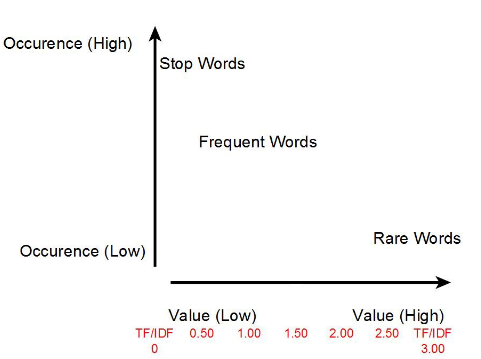
\includegraphics[width=8cm]{Pictures/slika1.png}
\centering
\caption{Prikaz odnosa učestalosti pojavljivanja reči i njihovog značaja.}
\end{figure}

Pošto nam je cilj da se bavimo obradom prirodnih jezika, za tako nešto možemo iskoristiti $nltk$ (engl. \em{The Natural Language Toolkit}). On predstavlja skup biblioteka i programa za simboličko i statističko procesiranje prirodnih jezika, konkretno engleskog jezika. Predstavlja vodeću platformu za izradu $Python$ programa za rad sa prirodnim jezikom, pa tako sadrži skup biblioteka za procesiranje teksta pri klasifikaciji, tokenizaciju, izvlačenje korena reči(engl. \em{stemming}), tagovanje, parsiranje itd. Stemeri (engl. \em{stemmers}) uklanjaju morfološke prefikse, sufikse i infikse iz reči, kako bi ostala samo srž. Postoji više različitih vrsta stemera, od kojih će prvi biti predstavljen $SnowballStemmer$, koji podržava naredne jezike: danski, holandski, engleski, finski, francuski, nemački, mađarski, italijanski, norverški, portugalski, rumunski, ruski, španski i švedski.\\\\
Kada hoćemo da vršimo klasifikaciju, to možemo učiniti pomoću više različitih klasifikatora koje nam nudi $sklearn$, kao što su:
\begin{itemize}
\item KNeighborsClassifier - ima višestruke primene u finansijama, zdravstvu, političkim naukama, detekciji rukopisa, prepoznavanju slika i videa, itd.. Koristi se i za klasifikaciju i za regresiju i bazira se na pristupu sličnosti objekata. $K$ predstavlja broj najbližih suseda. Ako je $K=1$, onda za algoritam kažemo da je samo algoritam najbližeg suseda (engl. \em{nearest neighbor algorithm}).
\item SGDClassifier - Stohastički gradijentni spust (engl. \em{Stochastic Gradient Descent-SGD}) je jednostavan, ali veoma efikasan pristup, čije se prednosti ogledaju u efikasnosti, jednostavnoj implementaciji, a mane su mu što zahteva određeni broj parametara (npr. regularizacioni parametar, broj iteracija) i osetljiv je na skaliranje objekata. 
\item MultinomialNB - Naivni Bajesof klasifikator (engl. \em{Naive Bayes classifier}) for multinomial models) je pogodan za klasifikaciju diskretnih objekata. 
\end{itemize}

\begin{figure}[t]
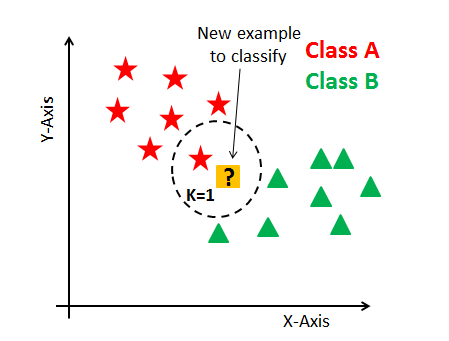
\includegraphics[width=8cm]{Pictures/slika2.png}
\centering
\caption{Prikaz K-najbližih suseda.}
\end{figure}
\newpage
\subsubsection{Predikcija kategorije teksta}
\begin{primer}
Naredni primer vrši predikciju kategorije teksta. Najpre se učitavaju podaci iz fajla $articles.csv$, u kome su podaci smešteni u obliku $kategorija, tekst$. Kolone koje čine fajl smeštamo u dve promenljive redom, $y$ i $texts$. Nakon toga, vrši se inicijalizacija vektorizatora za kreiranje TF-IDF matrice. Potom, primenjuje se neki od 3 klasifikatora:
\begin{itemize}
\item KNeighborsClassifier
\item SGDClassifier
\item MultinomialClassifier
\end{itemize}
Nakon fitovanja klasifikacionog modela, računarju se preciznosti na trening i test skupu, a potom se učitava test model i vrši se predikcija kategorije teksta. 
\end{primer}
\inputminted{python}{Codes/1/classifier.py}
Rezultat izvršavanja ovog programa je oblika:
\begin{lstlisting}
Train acc: 0.9871547848426461
Test acc: 0.968562874251497
['business']
['business', 'entertainment', 'politics', 'sport', 'tech']
[[0.38475301 0.09423106 0.28803524 0.11219421 0.12078647]]
\end{lstlisting}
\subsubsection{Latentna semantička analiza}
$LSA$ predstavlja način za particionisanje teksta korišćenjem statističkih modela upotrebe reči koji je sličan dekompoziciji sopstvenih vektora i analizi. Umesto da se samo fokusiramo na površne objekte kao što je učestalost reči, ovaj pristup obezbeđuje kvanitativnu meru semantičkih sličnosti među dokumentima baziranom na kontekstu reči. Dve glavne mane su sinonimi i polisemija. Sinonimija se odnosi na različite reči istog ili sličnog značenja. Sa druge strane, polisemija se odnosi na reči koje imaju više različitih značenja. $LSA$ pokušava da razreši ovaj tip problema, bez pomoći rečnika i sredstava na obradu prirodnih jezika, već korišćenjem matematičkih uzoraka koji postoje unutar podataka. To se postiže smanjenjem dimenzije koja se koristi da se dokument predstavi korišćenjem matematičke matrične operacije koja se naziva singularna dekompozicija (engl. SVD - Singular Value Decomposition).

SVD dekompozicija razbija bilo koju matricu $A$ na $A=U*S*V'$. Ako bismo bliže pogledali matricu $S$, videli bismo da je $S$ matrica forme, takve, da se sastoji od matrice $D$, koja na dijagonali sadrži sve $\sigma$, koje predstavljaju singularne vrednosti. Broj ovih singularnih vrednosti nam govori o rangu matrice $A$. Možemo pronaći aproksimaciju redukovanog ranga (engl. \em{truncated SVD} ili \em{LSA}) za $A$ tako što postavimo sve, osim prvih $k$ najvećih singularnih vrednosti na nulu, a potom koristimo samo prvih $k$ kolona matrica $U$  $V$. Ovaj postupak vršimo kako bismo izvršili redukciju dimenzionalnosti. Suprotno PCA, ovaj estimator ne centrira podatke pre izračunavanja singularne dekompozicije, što mu omogućava da radi efikasno sa retkim matricama (dostupnim kroz modul $scipy.sparse$). Konkretno, truncated SVD radi nad matricama sa brojevima termova (engl. \em{term count}) ili nad $tfidf$ matricama. U kontekstu ovih drugih, postupak je poznat kao latentna semantička analiza (engl. \em{latent semantic analysis-LSA}).\\\\
\begin{primer}
Ovaj primer vrši klasifikaciju novinskih članaka. Najpre se učitavaju podaci iz fajla $articles.csv$, u kome su podaci smešteni u obliku $kategorija, tekst$. Kolone koje čine fajl smeštamo u dve promenljive redom, $y$ i $texts$. Nakon toga, vrši se inicijalizacija vektorizatora za kreiranje TF-IDF matrice. Potom se vrši LSA.

\inputminted{python}{Codes/2/0-lsa.py}
Rezultat izvršavanja ovog programa predstavlja skup reči sa najvećim težinama po komponentama oblika:
\begin{lstlisting}
Component 182

('scottish', 0.09168672123398844)
('play', 0.08953887985792805)
('age', 0.08291233924728324)
('ethnic', 0.08288040224246893)
('murder', 0.08153061624591648)
('edward', 0.07253791078410225)
('develop', 0.07211813150850585)
('foster', 0.07116597034292958)
('minor', 0.07032073815220793)
('sentenc', 0.06973781343683193)
\end{lstlisting}
\end{primer}

\subsubsection{Web Scraping} 
Da bismo prikupili neke informacije sa veb stranica,a želimo to da uradimo na jednostavan način, potreban nam je program koji bi automatski izdvojio informacije od interesa i izvršio to izdvajanje za nas. Ovakav program naziva se skrejper (engl. \em{scraper}). On obilazi određenu vezu (ili, još češće, više veza na stranicama) i izdvaja željene informacije. Takav jedan program bio bi nam, na primer, potreban kako bismo popunili neki $.csv$ fajl u koji bismo mogli da smestimo neke novinske članke. Da bismo tako nešto postigli, moramo za svaku $.html$ stranicu koju posetimo: da izdvojimo relevantne informacije i da nađemo linkove ka ostalim. Kako bismo to uradili moramo koristiti regularne izraze i $re$ biblioteku koja nam omogućava rad sa njima. Da bismo uopšte mogli da $"$dovučemo$"$ stranice moramo koristiti $urllib.request$. \\
Urllib je paket koji sadrži nekoliko modula za rad sa URL-ovima:
\begin{itemize}
\item $urllib.request$ - za otvaranje i čitanje URL-ova,
\item $urllib.error$ - sadrži izuzetke koji se mogu javiti korišćenjem urllib.request,
\item $urllib.parse$ - za parsiranje URL-ova i 
\item $urllib.robotparser$ - za parsiranje $robots.txt$ fajlova.
\end{itemize}
Osim toga, u slučaju, da je neki sajt na ćirilici, a 
\begin{primer}
Naredni primer upravo vrši opisani postupak.


\inputminted{python}{Codes/2/1-scraper.py}

\begin{lstlisting}
/rss/
/scc/pretraga
/scc/rubrika/1/Svet
/scc/rubrika/2/Politika
/scc/rubrika/3/Drustvo
/scc/rubrika/4/Pogledi
/scc/rubrika/5/Hronika
/scc/rubrika/6/Ekonomija
/scc/rubrika/7/Kultura
/scc/rubrika/9/Srbija
/scc/rubrika/10/Beograd
/scc/rubrika/8/Sport
/scc/rubrika/29/Region
/scc/sarena-strana
/scc/rubrika/396/Magazin
/scc/rubrika/34/Moj-zivot-u-inostranstvu
/scc/satires/index
/scc/rubrika/1060/TV-revija
/scc/rubrika/1073/Tema-nedelje
/scc/clanak/414061/Slucaj-revizora-Sretenovica
clanak:
/scc/autor/913/Jovana-Rabrenovic
/scc/clanak/414064/Vlada-Crne-Gore-Srusicemo-crkvu-na-Rumiji
clanak:
/scc/clanak/414066/SAD-nisane-Rusiju-a-gadaju-Kinu
clanak:
/scc/autor/854/Jelena-Stevanovic
/scc/clanak/414096/Putin-Nas-odgovor-na-americke-rakete-u-Evropi-bice-brz-i-efikasan
clanak:
/scc/clanak/414059/U-rukama-ucenika-umesto-olovaka-cigarete
clanak:
/scc/clanak/414086/Sport/Ubedljiva-pobeda-Liverpula-protiv-Zvezde
clanak:
/scc/rubrika/49/Fudbal
/scc/clanak/414069/Oluja-krivac-za-rakete-ispaljene-iz-Gaze-na-Izrael
clanak:
/scc/clanak/414062/Zima-ce-biti-blaga-sa-malo-padavina
clanak:
/scc/clanak/414057/Humorom-protiv-straha
clanak:
/scc/clanak/414071/Pojacana-prodaja-novih-automobila
clanak:
/scc/clanak/414097/Sport/Kosarka/Dabl-dabl-Bjelice-u-pobedi-Kingsa-nad-Memfisom
clanak:
/scc/rubrika/50/Kosarka
/scc/clanak/414093/Americki-avion-predvodio-dronove-u-napadu-na-rusku-bazu-u-Siriji
\end{lstlisting}
\end{primer}

\newpage
\subsubsection{PageRank algoritam}
Naredni primer odnosi se na tzv. PageRank algoritam, odnosno, algoritam za rangiranje stranica. Ovaj algoritam je originalno objavljen od strane ljudi koji su učestvovali u kreiranju Google-a, Sergeja Brina i Lari Pejdža i smatra se odgovornim za njegov rani uspeh. Funkcioniše tako što stranice posmatra kao čvorove u grafu, a veze između stranica kao grane i potom obezbeđuje globalno rangiranje stranica na webu (čvorova u grafu). Za pretraživače obezbeđuje rangiranje stranica nezavisno od upita. Glavna pretpostvka ovog algoritma je da je svaka veza od stranice $a$ ka stranici $b$ glas od stranice $a$ za stranicu $b$. Bitno je naglasiti da nije svaki glas jednake težine. Težine dodeljuje PageRank algoritam na osnovu početnog čvora. Posmatrajmo primer sa slike \ref:pr1.

\begin{figure}[t]
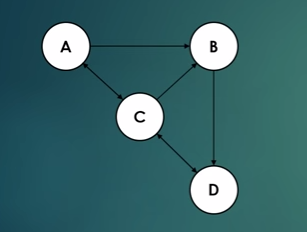
\includegraphics[width=8cm]{Pictures/pr1.png}
\centering
\caption{Prikaz grafa. A, B, C i D predstavljaju stranice.}
\end{figure}

 
\begin{primer} 
\end{primer}


\section{Eksperimenti}
\label{sec:prvi}



\section{Zaključak}
\label{sec:zakljucak}

\addcontentsline{toc}{section}{Literatura}
\appendix
\bibliography{seminarski} 
\bibliographystyle{plain}

\end{document}
